\subsection{Laplace Models}
In this section, we look at examples where we can apply the Laplace models.

Recall that in the Laplace model, for a subset $A \subseteq \Omega$ we have 
\begin{align*}
  \IP[A] = \frac{\abs{A}}{\abs{\Omega}}
\end{align*}

\begin{ex}[Hat Problem]
  We distribute $n$ hats to $n$ people. What is the probability that nobody receives their own hat.
  We set our event space $\Omega$ to be the set of all permutations $S_n$. Note that $\abs{S_n} = n!$

  For each $i \in \{1, \ldots, n\}$, let $A_i$ be the set of permutations that have $i$ as a fixed point.
  \begin{align*}
    A_i = \{\omega \in \Omega \big\vert \omega(i) = i\}
  \end{align*}
  If we set $A$ to be the permutations that have any fixed point, then by Lemma \ref{lem:IP-properties}
  \begin{align*}
    \IP[A] 
    &= 
    \IP\left[\bigcup_{i=1}^{n}A_i \right] 
    = \sum_{k=1}^{n} (-1)^{k+1} \sum_{1 \leq i_1< \ldots <i_k \leq n} \IP \left[
      A_{i_1} \cap \ldots \cap A_{i_k}
    \right]\\
    &= \sum_{k=1}^{n} (-1)^{k+1} \underbrace{\binom{n}{k} \frac{(n-k)!}{n!}}_{= \frac{1}{k!}} = - \sum_{k=1}^{n} \frac{(-1)^{k}}{k!}
  \end{align*}
  where we used the fact that there are $\binom{n}{k}$ ways to chose $k$ indices $i_{1}, \ldots, i_{k}$ and the probability that a random permutation fixes these $k$ points is $\frac{(n-k)!}{n!}$.

  So in the event that $n \to \infty$, the probability that there are no fixed points is
  \begin{align*}
    \IP[A^{c}] = 1 - \IP[A] = 1 + \sum_{k=1}^{n} \frac{(-1)^{k}}{k!} \stackrel{n \to  \infty}{\longrightarrow} e^{-1}
  \end{align*}

\end{ex}

\begin{ex}[Urn problems]
In an Urn we have $N$ numbered balls, $K$ of which are coloured red and $N-K$ white.
We take a sample of $n$ balls (with or without putting them back).
If we set $\omega_i$ to be the number that is picked at the $i$-th step, then the event space $\Omega$ is
\begin{itemize}
  \item With putting back: $\Omega_1 = \{(\omega_1, \ldots,\omega_n) \big\vert 1 \leq \omega_i \leq N\}$
  \item Without putting back: $\Omega_2 = \{(\omega_1, \ldots,\omega_n) \big\vert 1 \leq \omega_i \leq N, \omega_i \neq \omega_j  \text{ for } i \neq j\}$
\end{itemize}
Then set $\IP_i$ corresponding to an equal distribution on $\Omega_i$. We're interested in the distribution of the random variable $X$, which measures the number of picked balls that are red.
And let $A_{i,k}$ to be the number of samples that have exactly $k$ red balls.
\begin{align*}
  A_{i,k} = \{\omega \in  \Omega_i \big\vert \abs{\{1 \leq \omega_j \leq K\}} = k\}
\end{align*}
then the probability is simply $\IP_i[X = k] = \abs{A_{i,k}}/\abs{\Omega_i}$ and we just have to find out the size of these sets.
\begin{itemize}
  \item If the balls are returned into the Urn ($i=1$) we have that $\abs{\Omega_1} = N^{n}$, so if we set $p = \frac{K}{N}$ to be the proportion of red balls we have
    \begin{align*}
      \abs{A_{1,k}} &= K^{k}(N-K)^{n-k} \binom{n}{k}\\
      \implies \IP_1[X = k] &= \binom{n}{k} p^{k}(1 - p)^{n-k}
    \end{align*}
    This is called the \textbf{Binomial distribution} with parameters $n$ and $p$.

    \begin{figure}[h]
    \centering
    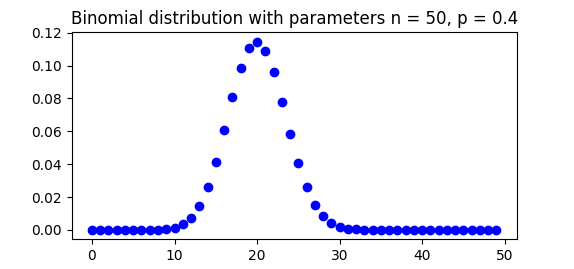
\includegraphics[width=0.5\textwidth]{./img/binomial.png}
    \caption{Plot of the Binomial distribution with parameters $n = 50, p = 0.4$. \texttt{./src/binomial.py}}
    \end{figure}
  \item For $i = 2$ we have
    \begin{align*}
      \abs{\Omega_2} &= N \cdot (N-1) \dots (N - n + 1) = \binom{N}{n}n!\\
      \abs{A_{2,k}} &= K(K-1) \dots (K-k+1) \cdot (N-K)(N - K - 1) \dots (N-K - (n-k) + 1) \binom{n}{k}\\
                    &= \binom{K}{k} \binom{N-K}{n-k}n!
    \end{align*}
    and it follows that
    \begin{align*}
      \IP_2[X = k] = \frac{\binom{K}{k} \binom{N-K}{n-k}}{\binom{N}{n}}
    \end{align*}
    which is called the \textbf{hypergeometric} distribution with parameters $n,N,K$
\end{itemize}
Notice that for $p= \frac{K}{N}$ constant and $n$ fixed, the hypergeometric distribution converges to the binomial distribution for $N,K$ large enough because the removal of each ball has less and less effect on the probability to chose a red ball at any step.
\end{ex}


%\subsection{Random walks}
%Consider a particle moving in a one-dimensional grid $\Z$ that startsat the origin $0$ and can take a step to the right or to the left with equal probability $\frac{1}{2}$.
%
%For a fixed $N \in \N$ let $\Omega$ be the set of all binary sequences of length $N$
%\begin{align*}
  %\Omega = \{\omega = (x_1, \ldots, x_N \big\vert x_i \in \{+1, -1\}\}
%\end{align*}


